\documentclass[20pt,margin=1in,innermargin=-4.5in,blockverticalspace=-0.25in]{tikzposter}
\geometry{paperwidth=42in,paperheight=30in}
\usepackage[utf8]{inputenc}
\usepackage{csquotes}
% \usepackage[estonian]{babel}
\usepackage{amsmath}
\usepackage{amsfonts}
\usepackage{amsthm}
\usepackage{amssymb}
\usepackage{mathrsfs}
\usepackage{graphicx}
\usepackage{adjustbox}
\usepackage{enumitem}
\usepackage{xcolor}
\usepackage[backend=biber,style=numeric]{biblatex}
\usepackage{Adjuntos/upj-theme}



\usepackage{mwe} % for placeholder images

\addbibresource{Adjuntos/refs.bib}

% set theme parameters
\tikzposterlatexaffectionproofoff
\usetheme{UPJTheme}
\usecolorstyle{UPJStyle}

\usepackage[scaled]{helvet}
\renewcommand\familydefault{\sfdefault} 
\renewcommand{\vec}[1]{\bm{#1}}
\newcommand{\Tr}{\text{Tr}}
\usepackage[T1]{fontenc}

\title{Road to the Future: Identifying Impacts of Roads on Education in Colombia}
\author{\textbf{Jaime Polanco}\textsuperscript{1} 
% and \textbf{Jane Smith}\textsuperscript{2} % Add 2nd author
}
\institute{\textsuperscript{1}  School of Economics and Management Sciences\\
                              Pontifical Xavierian University
            }
\titlegraphic{
\includegraphics[width=0.20\linewidth]{Adjuntos/logo.jpg}}

% begin document
\begin{document}
\maketitle
\centering
\begin{columns}
    \column{0.32}
    
    \block{Pregunta de investigación y contribución}
    {
    \justifying
Pregunta de investigación:
    \begin{center}
        ¿Cómo puede el desarrollo de infraestructura vial impactar la educación en Colombia?
    \end{center}
Contribución:
\begin{itemize}
    \item[] \justifying En este estudio pretendo aportar a la literatura  \textbf{evidencia del desarrollo en educación generado por la infraestructura vial en Colombia.}\\
\end{itemize}
    }
    
    \block{Contexto}{
    Este estudio requiere de información central, que en contexto se determina como:
\begin{itemize}
\justifying
    \item Red vial. La red vial en Colombia, ha tenido un lento crecimiento en las ultimas décadas. Para este estudio se tomara en cuenta las vías Tipo 1 ( alrededor 20mil Km), tipo 2 (alrededor de 3mil Km) y tipo 3 (alrededor de 6mil Km), las cuales se caracterizan por el estado de la superficie, el número de carriles y su accesibilidad. 
    \item Saber 11. Para finalizar la educación secundaria, se presenta el examen estandarizado de educación secundaria de grado 11, conocido como examen saber 11 (Antes conocido como ICFES) (8942 escuelas del 2006 al 2020). 
    \item Saber PRO.  los estudiantes de ultimo año de educación superior presentan de forma obligatoria el examen conocido como Saber Pro (Antes conocido como ECAES)  desde el año 2006, este suele ser un indicador que permite determinar que el estudiante accedió y termino estudios de educación superior.  
    %summary statistics
\end{itemize}
\caption{Relacion entre la mediana del examen estandarizado Saber 11 a nivel departamental con las vias tipo 1, tipo 2, y tipo 3 (linea roja) }
\centering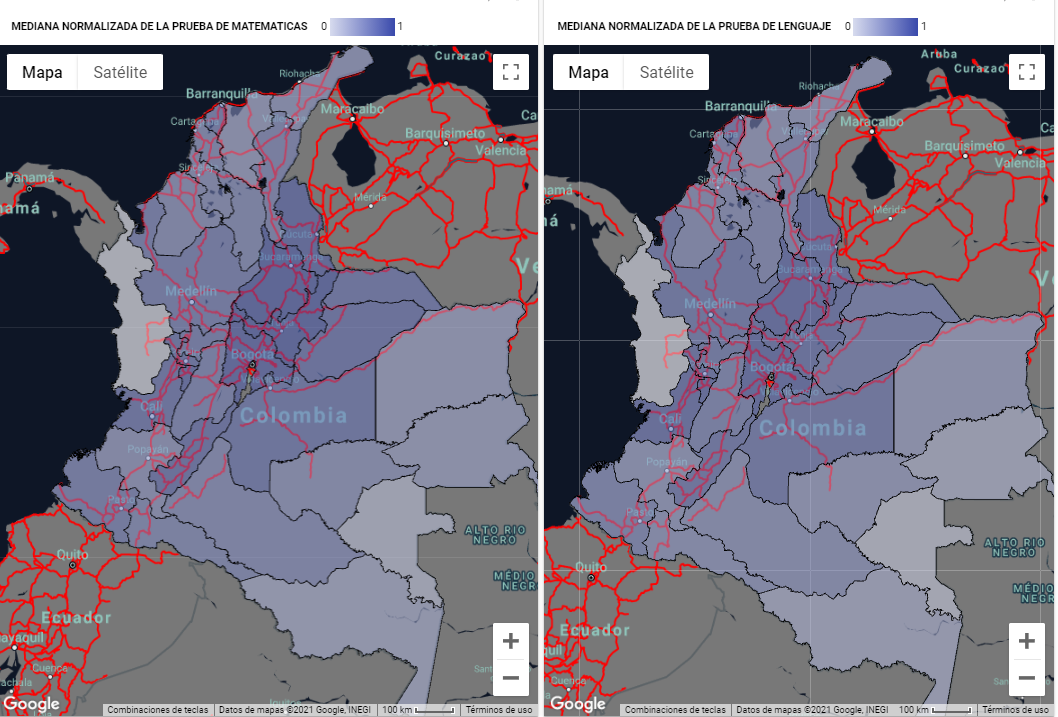
\includegraphics[scale=1]{Adjuntos/Roads_score.png}\\
\small\url{https://datastudio.google.com/u/0/reporting/20b144d6-8b14-4b10-ae64-120e14222869/page/LC6ZC}
    }
    \column{0.36}
     \block{Resumen estadístico. }{

        El valor presente en la tabla indica la distancia media entre los colegios y la vía tipo 1 mas cercana, y entre paréntesis se representa la desviación estándar para dado indicador  
         \begin{center}
             \begin{tabular}{llll}
        \hline
                & \multicolumn{3}{c}{$Proximity_1$ between (in meters)}   
         
         \\
                                & 0-850                  & \textgreater{} 850    \\ 
        \hline
        Distance                & 350 \small{(255)}       & 11662 \small{(35406)} \\
        Elevation              & 1324 \small{(951)}      & 971 \small{(955)}      \\
        Temperature            & 19.8 \small{(5.3)}      & 21.84 \small{(5.5)}    \\
        Precipitation          & 9.1 \small{(9)}          & 7.9 \small{(7.8)}     \\
        Volumetric soil water  & 0.4 \small{(0.05)}      & 0.37 \small{(0.09)}    \\
        Leaf Area index HV     & 4.44 \small{(1.20)}     & 4.2 \small{(1.36) }    \\
        Score math             & 0.495 \small{(0.141)}   & 0.449 \small{(0.144)}  \\
        Score Lang             & 0.524 \small{(0.138)}   & 0.478 \small{(0.142)}  \\   
        N                       & 4262           & 4263         \\
        \hline
        \end{tabular}
         \end{center}

     
     }
    \block{Antecedentes}{
    
    \justifying
        El efecto de la infraestructura vial y transporte, se han discutido y documentado en la literatura, agrupándose en beneficios  productivos,en pobreza, en disminución del costo de transporte, en movilidad ocupacional intergeneralcional, en accesos a nuevos mercados, en desempeño académico, entre otros. 
    \begin{center}
        \begin{tabular}{lllp{14cm}}
            \cline{1-4}
            Autor & Año & Estrategia  & Se evalúa...    \\
            \cline{1-4}
            
            Luis Quintero et al. & WP &DiD, VI &   Impacto sobre el PIB por carreteras \\
            Franco et al.  & 2021 & OLS CS &   Impacto sobre el desarrollo a largo plazo en Perú del camino Inca \\
            Fernandez et al. & 2020 & IV &   Impacto de la ocupación inter-generacional, conducido por la construcción de lineas férreas en el siglo XIX  \\
            Adukia et al.  & 2020   &    FE    & Impacto sobre la educación de 115000 nuevas vías en India         \\
            Herskovic L   & 2020   &     DiD  & Impacto de una nueva linea de metro en Chile.   \\
            % Donaldson et al.   &  2018   & GEM &  \\
            Dustan et al.  &  2018   &  DiD, IV ro &  Impacto de la expansión de transporte público sobre selección de escuela. \\
            Hine et al.  &  2016   &  Theorical Review &  Revisión de la expansión vial rural sobre la reducción de la pobreza. \\

            \cline{1-4}
        \end{tabular}
    \end{center}
    }
\block{Lidiando con la endogeneidad de las vias}{ 
Las carreteras son endógenas, en tanto existen donde hay personas, es decir donde hay oferta y demanda de vías, por ende existen donde hay generación de riqueza, lo que conlleva unir ciudades ricas y educadas.
\begin{center}
\begin{equation*} 
\small{ RoadProximity_{c,m}  = \alpha_o + \alpha_1{Surface Geological Conditions}_c \cdot {Historical Conditions}_c  }
\end{equation*} 
\begin{equation} \label{eq:4}\small{ 
 + \alpha_2{Historical Conditions}_c + \alpha_3{Surface Geological Conditions}_c
    + \sum^{k}  \gamma_k X_{k,c,m}  + \eta_{c } 
    + \epsilon_c}
\end{equation}     
\end{center}

}
%%%%%%%%%%%%%%%%%%%%%% Tercera columna
\column{0.32}
\block{El instrumento se explica por}{

Las condiciones superficiales geológicas, estarán determinadas por los siguientes atributos, los cuales, no explican de forma directa la educación:

\begin{center}
\centering
\begin{tabular}{llll}
Dato & medida &    \\
Saturación superficial de agua  & $m^3/m^3$ \\
Proximidad a Frontera agrícola  & $m$ \\
Proximidad a zonas de exclusión    & $m$      \\
Precipitación  & $m$      \\
Evaporación de la vegetación   & $m$ \\
Altura sobre el nivel del mar   & $m$  \\
\end{tabular}
\end{center}

Las condiciones históricas, estarán determinadas por los siguientes atributos, los cuales, no explican de forma directa la educación:
\begin{center}
\centering
\begin{tabular}{llll}
Dato & medida &    \\
Distancia a asentamientos precolombinos & $m$ \\
En búsqueda de otros  & $etc$ \\
\end{tabular}
\end{center}
}
    \block{Efecto sobre la educación, mediano plazo}{
     \justifying
        \textbf{Hipótesis: } \centering\textit{Quienes estudiaron la secundaria en instituciones próximas a vías tienen mayor probabilidad de asistir y terminar un programa de educación universitaria.} \\~\\
        % Para el caso de resultados binarios, tales como responder si un alumno participa o no en la prueba, se estima un instrumento no lineal, tal que:
         \justifying{Por simplicidad se presenta la forma lineal:}

        
        \begin{equation} \label{eq:1}
        \small {
                  Participate_{SaberPro_{i,c,t+s,e}} =  \beta_0 +  \sum_{m = 1}^{3} 
                \beta_m \cdot \widehat{RoadProximity_{c,i,  m, t}} +
                       \sum ^{k}  \alpha_k X_{k,c} %+\eta_{c } + 
                    + \sigma_{  t}+ \lambda_{e}+
                      \varepsilon_{c,j,t}
        }
        \end{equation} 
         \begin{itemize}
    \footnotesize{\justifying{
        Donde:\\
        $Participate_{SaberPro_{i,c,t+s,e}} $ Refiere a una variable dicótoma, donde sera igual a 1, si el individuo $i$ que se graduó del colegio $c$ a la edad $e$, participo en las pruebas Saber-Pro en el tiempo $t+s$. \\
        $RoadProximity_{c,i,  m, t}$ Refiere a la distancia en metros espaciales del colegio $c$ a la vía $m$, en la cual, estudio el individuo $i$ en el tiempo $t$.\\
        $\sigma_{t}$ y $\lambda_{e}$ Refiere a los efectos fijos de periodo y edad respectivamente.\\
        $\varepsilon$ refiere al termino del error\\
        }}
         \end{itemize}    
    }
    
    \block{Efecto sobre la educación a corto plazo}{
     \justifying
        \textbf{Hipótesis: }   \centering{\textit{Existe un efecto de la infraestructura vial sobre el desempeño en educación secundaria de Colombia. }} \\ 
             \begin{equation}
              {
                                 Score_{c}^j = \beta_0 + 
                                \sum_{m = 1}^{3} 
                                \beta_m  \widehat{ RoadProximity_{c,  m} } +
                                \sum_{n = 1}^{k} 
                             \alpha_k X_{k,c}  + u_c 
                              }
             \end{equation}

        \begin{itemize}
    \footnotesize{\justifying{
        Donde:\\
        $Score_{c}^j $ refiere al outcome, definido como la mediana del puntaje  estandarizado  de la materia $j$  del colegio $c$, \\
        $\widehat{ RoadProximity_{c,  m} }$ refiere la variable instrumental de la distancia minima espacial de la via $m$ al colegio $c$,\\
        $\beta$ refiere los estimadores de la regresión de las variables de interés, \\
        $X$ refiere a las $k$ variables de control,  \\
        $\alpha$ refiere a los coeficientes de estimación de las $k$ variables de control y $u$ refiere al termino del error. 
        }}
        \end{itemize}         

    } 

    \block{Agradecimientos}{
    Agradezco a la Universidad Pontificia Javeriana por el apoyo científico, en especial a Oliver Pardo por su supervisión. 
    }
    
    % \block{References}{
    %     \vspace{-1em}
    %     \begin{footnotesize}
    %     \printbibliography[heading=none]
    %     \end{footnotesize}
    % }
\end{columns}
\end{document}